\documentclass[a4paper,10pt]{article}
\usepackage[utf8]{inputenc}
\usepackage[margin=1.5cm, bottom=2cm]{geometry}
\usepackage{fancyhdr}
\usepackage{enumitem}
\usepackage{xcolor}
\usepackage{makeidx}
\usepackage[most]{tcolorbox}
\newtcolorbox{osservazioni}{
  colback=gray!8,    % sfondo grigio chiaro
  colframe=white,      % nessun bordo
  arc=2mm,            % angoli smussati
  boxrule=0pt,        % spessore bordo 0
  fontupper=\footnotesize,
  left=2mm, right=2mm, top=2mm, bottom=2mm,
  before skip=7pt,   % niente spazio prima
  after skip=15pt     % niente spazio dopo
}
\newtcolorbox{osservazioni2}{
  colback=gray!8,    % sfondo grigio chiaro
  colframe=white,      % nessun bordo
  arc=2mm,            % angoli smussati
  boxrule=0pt,        % spessore bordo 0
  fontupper=\small,
  left=5mm, right=5mm, top=3mm, bottom=3mm,
  before skip=0pt,   % niente spazio prima
  after skip=30pt     % niente spazio dopo
}
\pagestyle{fancy}
\usepackage{tikz}
\usetikzlibrary{automata, positioning}
\pagestyle{fancy}

\usepackage{makeidx}

%%%%%%%%%%%%%%%%%%%
\newcommand{\EsercitazioneNum}{02}
\newcommand{\Data}{23/10/2025}
\newcommand{\DocType}{Esercitazione} % o "Eserciziario"
\newcommand{\FullTitle}{\DocType\ \EsercitazioneNum}

\newcommand{\Header}{
\noindent
  \small \textbf{Computabilità, Complessità e Logica - a.a. 2025/26} \hfill \textbf{\FullTitle} \\[0.2cm]
  \scriptsize Matteo Liotta, \texttt{matteo.liotta@studenti.units.it} \hfill \Data \\[0.2cm]
  \noindent\makebox[\linewidth]{\rule{\linewidth}{0.4pt}} \\[0.3cm]}

\newcommand{\NewPageHeader}{
  \vfill
  \noindent\makebox[\linewidth]{\rule{\linewidth}{0.4pt}}
  \newpage
  {\Header}
}
%%%%%%%%%%%%%%%%%%%

% Numero di pagina in basso al centro
\fancyhf{}
\fancyfoot[C] \thepage
\renewcommand{\footrulewidth}{0pt} % niente linea in basso
\renewcommand{\headrulewidth}{0pt} % niente linea in alto



\begin{document}
\footnotesize 

\noindent
\small \textbf{Computabilità, Complessità e Logica - a.a. 2025/26} \hfill \textbf{Approfondimento \EsercitazioneNum} \\[0.2cm]
\scriptsize Matteo Liotta, \texttt{matteo.liotta@studenti.units.it} \hfill \Data \\[0.2cm]

\noindent\makebox[\linewidth]{\rule{\linewidth}{0.4pt}} \\[1cm]


\noindent\Large \textbf{Approfondimento \EsercitazioneNum}: \textit{Risoluzione di un esercizio su Automi a Pila}\\[0cm]
%\\[0.4cm]

\small

\noindent\underline{\textbf{Esercizio}}\\[0.3cm]
Si scriva un automa a pila che riconosca il linguaggio su $\Sigma=\{a,b\}$:

$$L=\{w\#w'| w,w'\in\Sigma^*, \quad \exists i \in \mathbf{N} \quad t.c.\quad  w(i)=w'(i)\ \}$$


\noindent\underline{\textbf{Soluzione}}\\[0.3cm]
\noindent Il linguaggio indicato riconosce le parole per cui, quando scritte prima e dopo un simbolo di $\#$, ammettono un indice $i$, tale per cui in quella posizione le due parole solo uguali:
$$w(i)=w'(i)$$

\noindent L'idea per la soluzione impiega il non determinismo per \textbf{scegliere} la posizione \textit{$i$-esima} da controllare: sfruttando tale possibilità, considerato che possiamo ritenere accettata una parola per cui esiste almeno una \textit{computazione accettante}, possiamo considerare tutte le $i$ eseguendo tutte le computazioni parallele.\\

\noindent Svilupperemo, inoltre, un arco per ogni simbolo dell'alfabeto, così da identificare $|\Sigma|$ zone destinate alla gestione di ogni caso in cui controlliamo che l'i-esima posizione sia uguale (a un certo simbolo). 
Partiamo allora dal considerare che a partire da uno stato iniziale possiamo scommettere sulla lettera che verificherà l'uguaglianza, nel nostro caso o $a$ o $b$. I due casi si distinguono nella \textbf{lettera} che verrà scritta all'interno della \textbf{pila}, oltre che \textbf{al controllo finale}. Si noti che questa possibilità è garantita dalla finitezza dell'alfabeto $\Sigma$. 


    {
    \small
    \begin{center}
	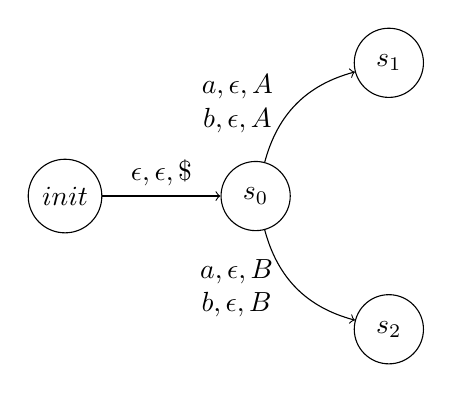
\begin{tikzpicture}
		
        \node[state, text=] (A) {$s_0$};
        \node[state, initial text=, left=1.5of A] (init) {$init$};
		\node[state] (B) [above right=1.5of A] {$s_1$};
		\node[state] (C) [below right=1.5of A] {$s_2$};

		\path[->] 
        (init) edge[above] node{$\epsilon, \epsilon,\$$} (A)
        (A) edge[left, bend left] node {$\begin{array}{c} a,\epsilon,A \\ b,\epsilon,A\end{array}$}  (B)
        (A) edge[left, bend right] node {$\begin{array}{c} a,\epsilon,B \\ b,\epsilon,B\end{array}$}  (C);       

    \end{tikzpicture}
    \end{center}
    }

Alla prima lettera letta, abbiamo inserito una $A$ o una $B$ nella pila. Possiamo farlo più volte:

    {
    \small
    \begin{center}
	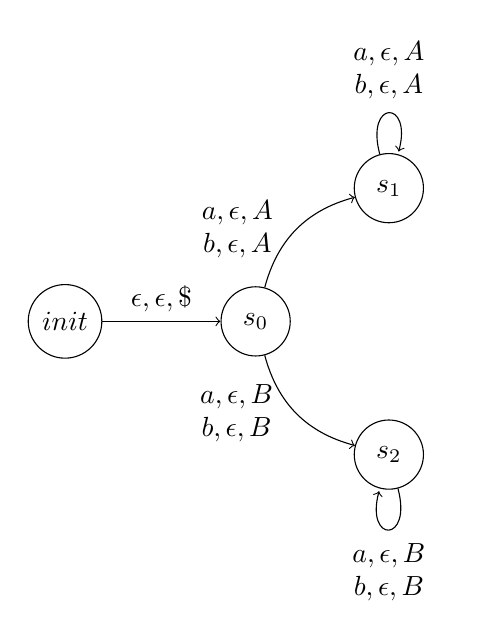
\begin{tikzpicture}
		
        \node[state, text=] (A) {$s_0$};
        \node[state, initial text=, left=1.5of A] (init) {$init$};
		\node[state] (B) [above right=1.5of A] {$s_1$};
		\node[state] (C) [below right=1.5of A] {$s_2$};

		\path[->] 
        (init) edge[above] node{$\epsilon, \epsilon,\$$} (A)
        (A) edge[left, bend left] node {$\begin{array}{c} a,\epsilon,A \\ b,\epsilon,A\end{array}$}  (B)
        (A) edge[left, bend right] node {$\begin{array}{c} a,\epsilon,B \\ b,\epsilon,B\end{array}$}  (C)        
        (B) edge[left, loop above] node {$\begin{array}{c} a,\epsilon,A \\ b,\epsilon,A\end{array}$}  (B)        
        (C) edge[left, loop below] node {$\begin{array}{c} a,\epsilon,B \\ b,\epsilon,B\end{array}$}  (C);        


    \end{tikzpicture}
    \end{center}
    }

\noindent Ad ogni lettera che viene letta, a questo punto, viene inserito un simbolo nella pila: la pila \textit{rappresenta un contatore, poiché contiene un simbolo per ciascuna delle lettere lette della parola} $w$. Come possiamo allora selezionare la $i$ per controllare l'uguaglianza? L'idea è che non deterministicamente possiamo saltare a uno stato che ferma la lettura della parola $w$:

\NewPageHeader


    {
    \small
    \begin{center}
	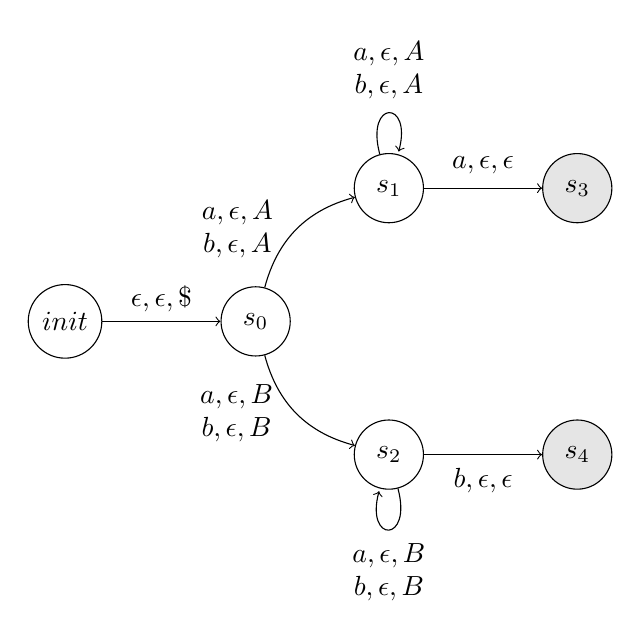
\begin{tikzpicture}
		
        \node[state, text=] (A) {$s_0$};
        \node[state, initial text=, left=1.5of A] (init) {$init$};
		\node[state] (B) [above right=1.5of A] {$s_1$};
		\node[state] (C) [below right=1.5of A] {$s_2$};
        \node[state] (D) [right=1.5of B, fill=black!10] {$s_3$};
		\node[state] (E) [right=1.5of C, fill=black!10] {$s_4$};

		\path[->] 
        (init) edge[above] node{$\epsilon, \epsilon,\$$} (A)
        (A) edge[left, bend left] node {$\begin{array}{c} a,\epsilon,A \\ b,\epsilon,A\end{array}$}  (B)
        (A) edge[left, bend right] node {$\begin{array}{c} a,\epsilon,B \\ b,\epsilon,B\end{array}$}  (C)        
        (B) edge[left, loop above] node {$\begin{array}{c} a,\epsilon,A \\ b,\epsilon,A\end{array}$}  (B)        
        (C) edge[left, loop below] node {$\begin{array}{c} a,\epsilon,B \\ b,\epsilon,B\end{array}$}  (C)        
        (B) edge[above] node {$\begin{array}{c} a,\epsilon,\epsilon\end{array}$}  (D)
        (C) edge[below] node {$\begin{array}{c} b,\epsilon,\epsilon\end{array}$}  (E);        

    \end{tikzpicture}
    \end{center}
    }

\noindent Proprio la possibilità di saltare in ogni momento concede alla macchina la possibilità di eventualmente considerare ogni posizione. Da lì non siamo interessati alle altre parole, quindi si arriva al $\#$ smettendo di incrementare il contatore:

    {
    \small
    \begin{center}
	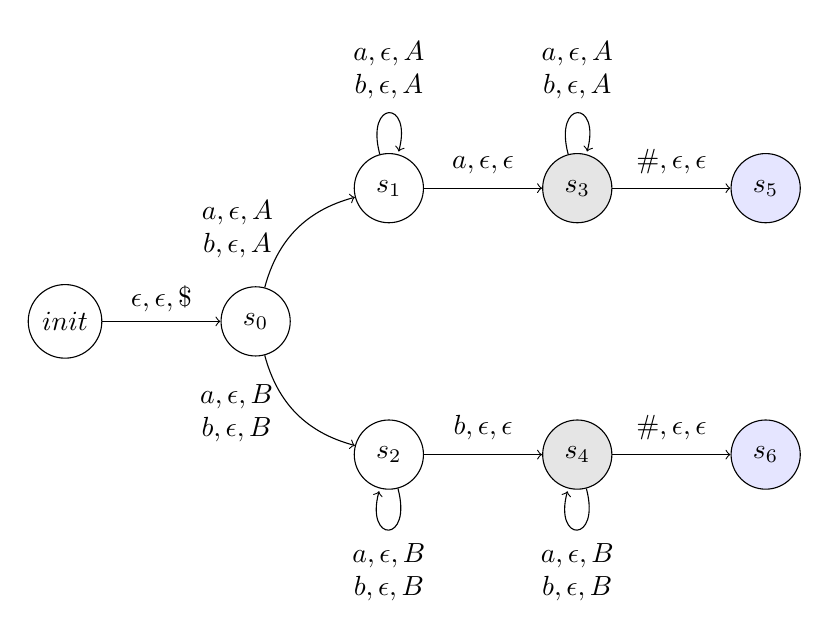
\begin{tikzpicture}
		
        \node[state, text=] (A) {$s_0$};
        \node[state, initial text=, left=1.5of A] (init) {$init$};
		\node[state] (B) [above right=1.5of A] {$s_1$};
		\node[state] (C) [below right=1.5of A] {$s_2$};
        \node[state] (D) [right=1.5of B, fill=black!10] {$s_3$};
		\node[state] (E) [right=1.5of C, fill=black!10] {$s_4$};
        \node[state] (F) [right=1.5of D, fill=blue!10] {$s_5$};
		\node[state] (G) [right=1.5of E, fill=blue!10] {$s_6$};

		\path[->] 
        (init) edge[above] node{$\epsilon, \epsilon,\$$} (A)
        (A) edge[left, bend left] node {$\begin{array}{c} a,\epsilon,A \\ b,\epsilon,A\end{array}$}  (B)
        (A) edge[left, bend right] node {$\begin{array}{c} a,\epsilon,B \\ b,\epsilon,B\end{array}$}  (C)        
        (B) edge[left, loop above] node {$\begin{array}{c} a,\epsilon,A \\ b,\epsilon,A\end{array}$}  (B)        
        (C) edge[left, loop below] node {$\begin{array}{c} a,\epsilon,B \\ b,\epsilon,B\end{array}$}  (C)        
        (B) edge[above] node {$\begin{array}{c} a,\epsilon,\epsilon\end{array}$}  (D)
        (D) edge[left, loop above] node {$\begin{array}{c} a,\epsilon,A \\ b,\epsilon,A\end{array}$}  (D)       
        (C) edge[above] node {$\begin{array}{c} b,\epsilon,\epsilon\end{array}$}  (E)
        (E) edge[below, loop below] node {$\begin{array}{c} a,\epsilon,B \\ b,\epsilon,B\end{array}$}  (E)           
        
        (D) edge[above] node {$\begin{array}{c} \#,\epsilon,\epsilon\end{array}$}  (F)
        (E) edge[above] node {$\begin{array}{c} \#,\epsilon,\epsilon\end{array}$}  (G);

    \end{tikzpicture}
    \end{center}
    }

\noindent A questo punto, essendo pronti a leggere la seconda parola, possiamo scaricare la pila, per ogni lettura, fino a raggiungere la $i$-1 esima lettera della parola $w'$.


    {
    \small
    \begin{center}
	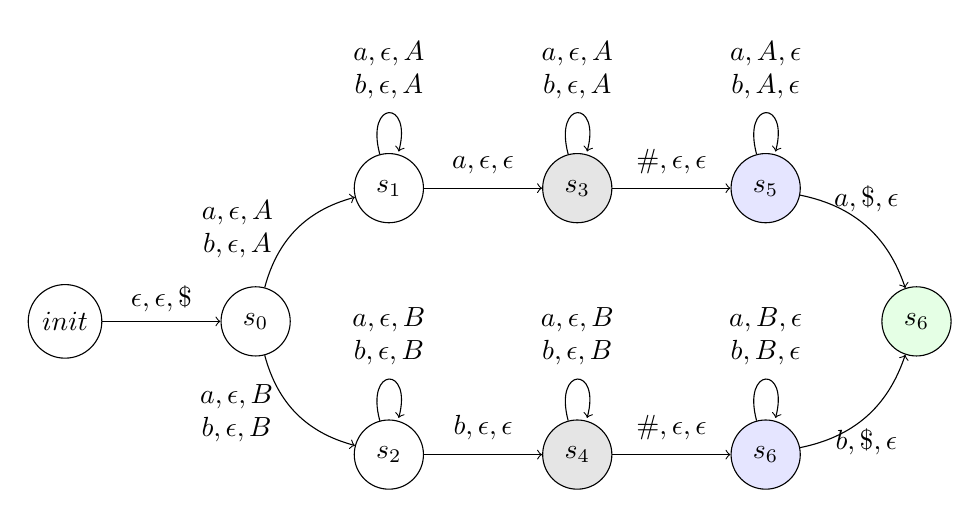
\begin{tikzpicture}
		
        \node[state, text=] (A) {$s_0$};
        \node[state, initial text=, left=1.5of A] (init) {$init$};
		\node[state] (B) [above right=1.5of A] {$s_1$};
		\node[state] (C) [below right=1.5of A] {$s_2$};
        \node[state] (D) [right=1.5of B, fill=black!10] {$s_3$};
		\node[state] (E) [right=1.5of C, fill=black!10] {$s_4$};
        \node[state] (F) [right=1.5of D, fill=blue!10] {$s_5$};
		\node[state] (G) [right=1.5of E, fill=blue!10] {$s_6$};
        \node[state] (ok) [right=7.5of A, fill=green!10] {$s_6$};


		\path[->] 
        (init) edge[above] node{$\epsilon, \epsilon,\$$} (A)
        (A) edge[left, bend left] node {$\begin{array}{c} a,\epsilon,A \\ b,\epsilon,A\end{array}$}  (B)
        (A) edge[left, bend right] node {$\begin{array}{c} a,\epsilon,B \\ b,\epsilon,B\end{array}$}  (C)        
        (B) edge[left, loop above] node {$\begin{array}{c} a,\epsilon,A \\ b,\epsilon,A\end{array}$}  (B)        
        (C) edge[left, loop above] node {$\begin{array}{c} a,\epsilon,B \\ b,\epsilon,B\end{array}$}  (C)  
        
        (B) edge[above] node {$\begin{array}{c} a,\epsilon,\epsilon\end{array}$}  (D)
        (D) edge[left, loop above] node {$\begin{array}{c} a,\epsilon,A \\ b,\epsilon,A\end{array}$}  (D)       
        (C) edge[above] node {$\begin{array}{c} b,\epsilon,\epsilon\end{array}$}  (E)
        (E) edge[below, loop above] node {$\begin{array}{c} a,\epsilon,B \\ b,\epsilon,B\end{array}$}  (E)           
        
        (D) edge[above] node {$\begin{array}{c} \#,\epsilon,\epsilon\end{array}$}  (F)
        (E) edge[above] node {$\begin{array}{c} \#,\epsilon,\epsilon\end{array}$}  (G)

        (F) edge[left, loop above] node {$\begin{array}{c} a,A,\epsilon \\ b,A,\epsilon\end{array}$}  (F)    
        (G) edge[below, loop above] node {$\begin{array}{c} a,B,\epsilon \\ b,B,\epsilon\end{array}$}  (G)

        (F) edge[above,bend left] node {$\begin{array}{c} a,\$,\epsilon\end{array}$}  (ok)
        (G) edge[below, bend right] node {$\begin{array}{c} b,\$,\epsilon\end{array}$}  (ok);

        
    \end{tikzpicture}
    \end{center}
    }
\NewPageHeader
L'ultima transizione aggiunta serve a garantire che, quando la pila sarà vuota, l'unica lettura che possa portare alla lettera che garantisce la terminazione sia proprio quella su cui abbiamo scommesso. Ci si troverà d'innanzi alla $i$-esima lettera della seconda parola, $a$ o $b$ nel primo o nel secondo caso.\\

\noindent L'esercizio non è risolto però per l'intero linguaggio: poiché la macchina inserisce sempre una lettera nella pila, non è in realtà in grado di controllare anche l'uguaglianza nella prima posizione. Eppure, dovremmo anche gestire il caso in cui $i=1$.
Per farlo, l'idea è considerare anche $s_0$ uno stato in cui è possibile non deterministicamente effettuare la transizione, anche se purtroppo dobbiamo considerare altri stati, in quanto il contatore $i-1=1-1=0$ necessita la pila vuota e, usando gli altri archi, essa verrebbe riempita.

    {
    \small
    \begin{center}
	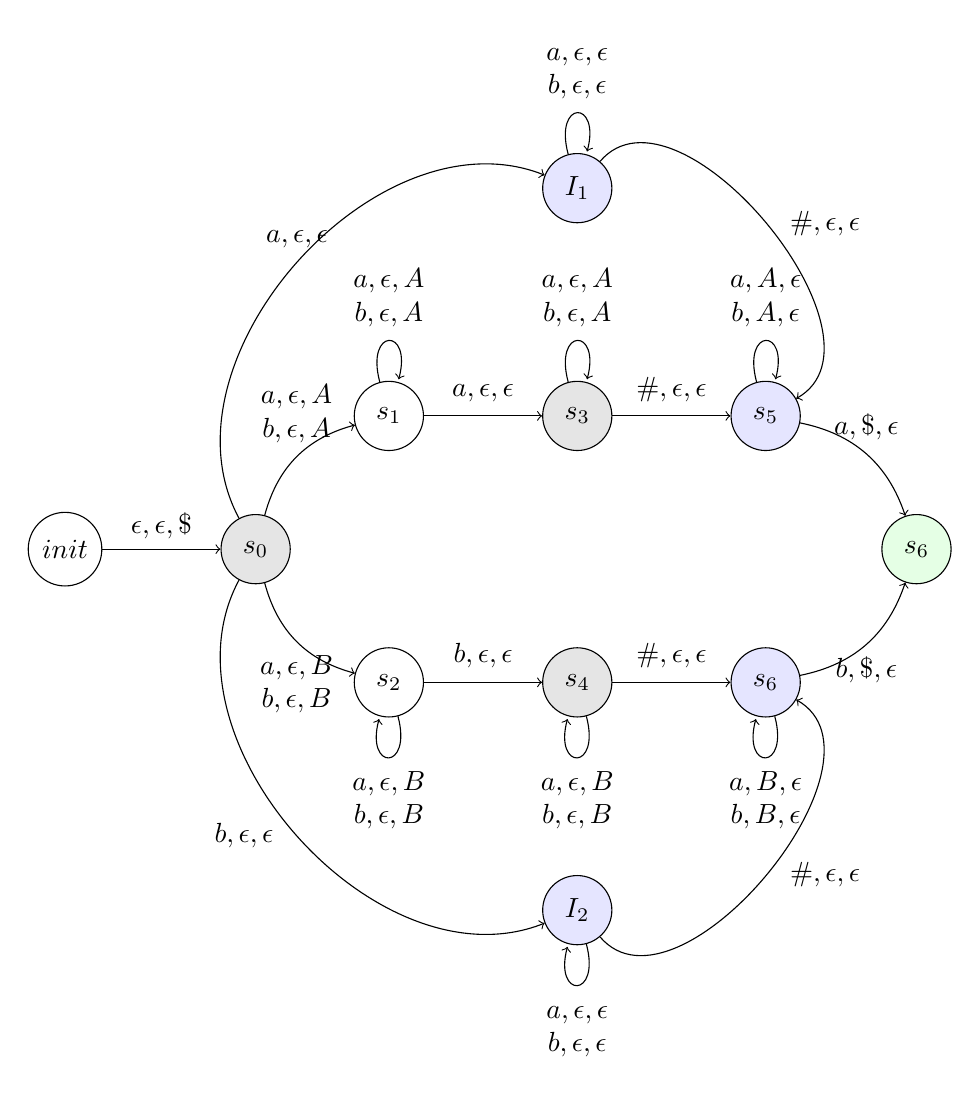
\begin{tikzpicture}
		
        \node[state, text=, fill=black!10] (A) {$s_0$};
        \node[state, initial text=, left=1.5of A] (init) {$init$};
		\node[state] (B) [above right=1.5of A] {$s_1$};
		\node[state] (C) [below right=1.5of A] {$s_2$};
        \node[state] (D) [right=1.5of B, fill=black!10] {$s_3$};
		\node[state] (E) [right=1.5of C, fill=black!10] {$s_4$};
        \node[state] (F) [right=1.5of D, fill=blue!10] {$s_5$};
		\node[state] (G) [right=1.5of E, fill=blue!10] {$s_6$};
        \node[state] (ok) [right=7.5of A, fill=green!10] {$s_6$};

        \node[state] (I1) [above=2of D, fill=blue!10] {$I_1$};
		\node[state] (I2) [below=2of E, fill=blue!10] {$I_2$};


		\path[->] 
        (init) edge[above] node{$\epsilon, \epsilon,\$$} (A)
        (A) edge[above, bend left] node {$\begin{array}{c} a,\epsilon,A \\ b,\epsilon,A\end{array}$}  (B)
        (A) edge[below, bend right] node {$\begin{array}{c} a,\epsilon,B \\ b,\epsilon,B\end{array}$}  (C)        
        (B) edge[left, loop above] node {$\begin{array}{c} a,\epsilon,A \\ b,\epsilon,A\end{array}$}  (B)        
        (C) edge[left, loop below] node {$\begin{array}{c} a,\epsilon,B \\ b,\epsilon,B\end{array}$}  (C)  
        
        (B) edge[above] node {$\begin{array}{c} a,\epsilon,\epsilon\end{array}$}  (D)
        (D) edge[left, loop above] node {$\begin{array}{c} a,\epsilon,A \\ b,\epsilon,A\end{array}$}  (D)       
        (C) edge[above] node {$\begin{array}{c} b,\epsilon,\epsilon\end{array}$}  (E)
        (E) edge[below, loop below] node {$\begin{array}{c} a,\epsilon,B \\ b,\epsilon,B\end{array}$}  (E)           
        
        (D) edge[above] node {$\begin{array}{c} \#,\epsilon,\epsilon\end{array}$}  (F)
        (E) edge[above] node {$\begin{array}{c} \#,\epsilon,\epsilon\end{array}$}  (G)

        (F) edge[left, loop above] node {$\begin{array}{c} a,A,\epsilon \\ b,A,\epsilon\end{array}$}  (F)    
        (G) edge[below, loop below] node {$\begin{array}{c} a,B,\epsilon \\ b,B,\epsilon\end{array}$}  (G)

        (F) edge[above,bend left] node {$\begin{array}{c} a,\$,\epsilon\end{array}$}  (ok)
        (G) edge[below, bend right] node {$\begin{array}{c} b,\$,\epsilon\end{array}$}  (ok)

        (A) edge[above,bend left=70] node {$\begin{array}{c} a,\epsilon,\epsilon\end{array}$}  (I1)
        (A) edge[left,bend right=70] node {$\begin{array}{c} b,\epsilon,\epsilon\end{array}$}  (I2)

        (I1) edge[left, loop above] node {$\begin{array}{c} a,\epsilon,\epsilon \\ b,\epsilon,\epsilon\end{array}$}  (I1)    
        (I2) edge[below, loop below] node {$\begin{array}{c} a,\epsilon,\epsilon \\ b,\epsilon,\epsilon\end{array}$}  (I2)

        (I1) edge[bend left=100, right] node {$\begin{array}{c} \#,\epsilon,\epsilon\end{array}$}  (F)
        (I2) edge[bend right=100, right] node {$\begin{array}{c} \#,\epsilon,\epsilon\end{array}$}  (G);
        

        
    \end{tikzpicture}
    \end{center}
    }
\vfill
\noindent\makebox[\linewidth]{\rule{\linewidth}{0.1pt}}
\end{document}
